\section{Problem Outline}
The problem this thesis is trying to solve is to select a number of songs given a predefined playlist so that the selected songs constitute a playlist similar to the predefined one. 

\section{Assumptions}
\begin{displayquote}
\textit{Without assumptions you cannot do machine learning} \\\\Ryan Adams
\end{displayquote}

The goal of the thesis is to generate playlists, similar to seed playlists choosen by the user. In order to do this there is a need for assumptions regarding playlists.

The first assumption for this thesis is that curated playlists, playlists made by professionals whose work is to create good playlists, suited for a specific context are suitable training data to create a model that generates playlists suited to the same playlist context.

The second assumption made is that features that belong to each track in a curated playlist contain enough information to create a representation of the context this curated playlist is made for.

The third assumption is that a playlist can be looked at as a good mixture of songs, i.e. there is an inherit variance in the playlist that defines it. This is a clear distinction from assuming that playlists only consist of songs similar to each other.


\section{Data}
From the Spotify hadoop cluster all available playlists where extracted and then filtered based upon whether they were created by Spotify playlist curators or not. Once playlists were filtered, feature data consisting of discrete values for genre, mood and tempo were added to each track within the selected subset of playlists.

\section{Pre-processing}
The selected data did contain track duplicates within playlists. These were removed as they would otherwise affect each playlist´s covariance of features.

\section{Exploratory Data Analysis}
To get an overview of whether features of tracks in a curated playlist relate to each other within the playlist correlation exploratory data analysis was made through plotting. More specifically correlation plots on a playlist level were made. The idea behind plotting correlations instead of covariances is that the magnitude of the correlation shows the strength of the linear relationship between features, while a covariance plot would be polluted should different features be on different ranges. By plotting correlations the problem of calculating correlations for features with zero variance, given a playlist context, emerged. Zero variance terms are a problem in the correlation setting as calculating the correlation for a zero variance term would imply dividing by zero, a mathematically undefined operation. This problem was solved by setting the correlation for feature relations with zero covariance to zero. It can be argued whether this is mathematically correct or not. But the approach can be motivated in this setting by the fact that plots are done to get an intuition of the data. A correlation of zero for features with zero covariance thus gives a better intuition of relationships in the data set compared to setting the correlation to one.

Performing plots of feature covariances of a playlist also shows whether there are linear realtionships among features in that playlist or not.

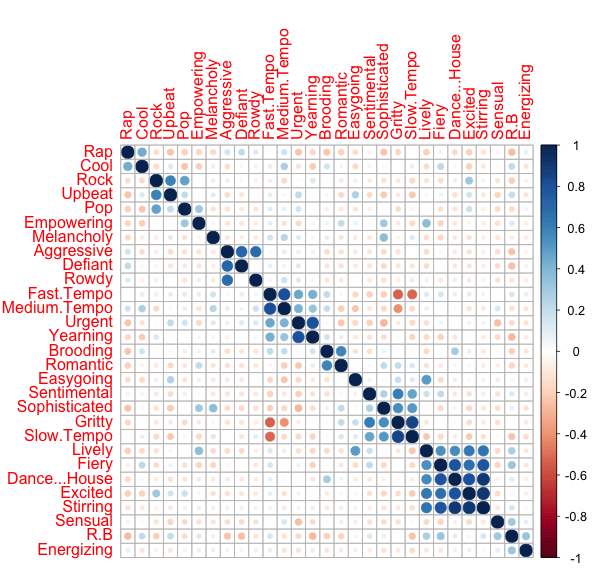
\includegraphics[scale=0.6]{images/0removedPlistFeaturePlot.png}

As we can see from the example plot above, there are clearly linear correlations among features for our example playlist.

\section{Learning Playlist Characteristics}
\begin{comment}
Motivate, why?
\end{comment}
Once that linear relationships have been spotted in the data the next step is to create a model that can learn the representation of a specific playlist. One simple approach to learning latent factors in data is principle components analysis, PCA.
Explaining the characteristics for a certain playlist context could be seen as equivalent of explaining the variance of features for tracks, given a curated playlist suited to the specific playlist context. Therefore extracting the main characteristics for a playlist context can be done by extracting the principal components, for the curated playlist representing that playlist context. It is reasonable to assume that the data that is modelled by PCA is not noise free, why PCA is performed up to a certain threshold for the variance explained and thus a dimensionality reduction is made. 
Using this approach extracting eigenvectors for the covariance matrix, rather than correlation matrix, is a motivated choice. The motivation behind this choice is that scaling the covariance matrix to a correlation matrix is a nonlinear transformation. If we want to use apply the principal components of a correlation matrix to the original data, then the original data need to undergo the same transform as transforming covariances to correlations. For a data set where each curated playlist makes up less than one percent of the total data it would be impractical to transform the original data over and over as we extract the principal components for each playlist context. Doing so would also not be feasible in terms of scalability. Using the covariance matrix for extraction of features is therefore motivated as the principal components of the covariance matrix can be directly related to the existing data.

\section{Handling zero variance terms}
Even though there are no zero variance terms in the whole data set, there are some terms that have zero variance within a certain curated playlists. These terms will not be handled by the principal components describing a playlist context, as principal components describe the variance of a playlist. Despite not being handled by the principal components zero variance terms might still have an important role in describing a playlist context. For example, if we have a curated jazz playlist then it is probably an important factor that all of the tracks in this playlist have a zero value for rap. The importance of this can be easily understood by imagining the opposite, what if those tracks would have a constant non-zero value for rap? Then a non-zero value for rap associated with jazz would be an important indicator for that playlist, why the absence must also be an important indicator.

\section{Selecting candidate songs for a playlist context}
The process of selecting candidate songs given a specific playlist context is an interesting and ambiguous problem without a given approach. Earlier work is focused mainly on item to item recommendation, i.e. recommending similar items of the same type given preferences for items of a certain times. But when it comes to selecting appropriate songs for a playlist context the items are of different kinds. The goal is to recommend songs, one type of item, given a playlist describing a playlist context, which is another type of item. 

One initial idea to select songs for a given playlist context could be that songs are either good candidates or not. This is a reasonable assumption, as for example for a rock classics playlist context then songs are either rock classics or not. Given that this is a binary classification problem, an efficient two class classifier might seem as a good idea at a glance. A support vector machine, SVM,  is an optimal two class classifier by definition, as a SVM maximizes the margin between classes\cite{cortes1995support}, and has the capability of multi class classification with for example the one versus all approach\cite{hsu2002comparison}. There is however one problem with support vector machines, or any classifier that requires training data within contextual playlist generation. The problem is that it is easy to define training data which labels a song as belonging or not belonging to a certain playlist. But it is hard to define what songs that belong to other playlists, than the one describing a specific playlist context, which are still relevant for that playlist context. For example a song belonging to a house Workout playlist may very well be a suitable candidate for a house party playlist. It is actually often the case that many songs belong to several playlists, describing different playlist contexts. Given this example a discriminative model turns out to be a bad fit for the problem this thesis is trying to solve. If a song belongs to a house party playlist then it is reasonable to assume that it would be outside the margin defining a house workout playlist if feeded to a SVM, even though this particular song might very well be a suitable match for the house workout playlist. This rules out the use of SVMs for the purpose of this thesis, as SVMs need to know the mapping between songs and playlist contexts to work. The same mapping that we are trying to find.

A second idea to selecting songs suitable for a specific playlist context would be to use centroid based clustering. The wikipedia definition of clustering is as follows: "clustering is the task of grouping a set of objects in such a way that objects in the same group (called a cluster) are more similar (in some sense or another) to each other than to those in other groups (clusters)". One could for example cluster all tracks in curated playlists and then simply assign each song that is not part of a curated playlist to the cluster providing the best fit for each track. But one problem is that there is not a one to one mapping between tracks and playlists, one playlist can contain many tracks and one track can belong to many playlists. This is different from clustering where each cluster consists of many points, but each point only belongs to one cluster, which yields centroid based clustering impropriate for the scope of this thesis. 

A third approach to finding candidate songs given a playlist context would be to tweak the normal usage of collaborative filtering. The common approach of collaborative filtering is to use a sparse matrix to infer the rating of items for one user given the ratings of similar users. What can be done instead is to use binary ratings and instead of inferring ratings for a user one could infer ratings for songs given a playlist. What this means is that playlists that contain the same songs as a playlist describing a playlist context one is interested in will be used to infer songs that are good matches for the specified playlist context. 

\subsection{Subspace method}
A last approach for track candidate selection would be to use the subspace method. Given that the principal components for a playlist, describing the variance of that playlist suited for a playlist context, are at hand, one can simply treat each track as a vector rather than a point. Each vector can then be projected into the principal component space for that playlist context. The underlying assumption is then that points that have a low relative change in magnitude under projection are well described by the characteristics defining the playlist context, and thus good candidates. Tracks that are not well described by the playlist context characteristics on the other hand, will change under projection and will therefore also have a high relative change in magnitude. There are however problems with this approach. Lets say that we have a playlist context that is defined by variance in the dimensions jazz, blues and rap and our vector space consists of the dimensions jazz, blues, rap and rock. If we then have a song that is characterized by jazz and blues only, then this song will go unchanged under projection. As the relative change in magnitude is none then this song will be suggested as a suitable candidate for the jazz, blues, rap playlist context. However a playlist context consisting of jazz, blues and rap is likely to be pretty peculiar and a song characterized by jazz and blues only is not likely to be a suitable match for such a playlist. Another problem would be songs that consists of zero values for all features, these songs would also go unchanged under any playlist context projection, but are not likely to be good candidates for all playlist contexts. Further, the subspace method is a linear transformation and it can be questioned if a linear transformation is powerful enough to describe the necessary mappings.

\section{First Track Manifold}
After studying linear relationships among features within playlists the study was extended to see if there were linear relationships among the ordering of songs as well. To do this the subspace method was used again. But instead of extracting the principal components for the variance of a playlist, the principal components describing the variance of all the start songs of all curated playlists were extracted. Once this was made a sample of songs from the curated playlist data set were projected into the first track manifold space created by the principal components of the first tracks. This was made to see if start tracks would have higher ranking, i.e. lower relative change in magnitude, than other tracks.

\section{Playlist Comparison}
As principal components were chosen to describe playlists, it is reasonable to assume that if principal components analysis works well for describing playlist characteristics, then the same approach should also work well for comparing playlists. Playlists were compared pairwise. To compare two playlists all eigenvectors from each playlist were multiplied by each other. By doing this the cosine measure of vector similarity for each pair of vectors was obtained. The problem with this approach is that it gives an unbalanced comparison. By simply looking at the similarity of eigenvectors implies that eigenvectors corresponding to low eigenvalues have the same importance as eigenvectors corresponding to high eigenvalues. For the reader uninitiated with eigenvalues this means that components explaining a high part of the characteristics of a playlist are regarded an equal importance as components explaining a low part of playlist characteristics. To remedy this problem the cosine score between eigenvectors from each playlist was scaled by the square root of the product of the corresponding eigenvalues. The result obtained from this multiplication was a matrix. To rank the similarity between these matrices some type of transformation from a matrix to a single value is needed. Several approaches were tested and are covered under the evaluation section.

\section{Approximate Nearest Neighbours}
OL
